\documentclass[11pt,a4paper]{article}
\usepackage[latin1]{inputenc}
\usepackage[swedish,english]{babel}
\usepackage{graphicx}
\usepackage{amsfonts}
\usepackage{amsmath}
\usepackage{amssymb}
\usepackage{algorithm}
\usepackage{algorithmic}
\usepackage{url}

\DeclareGraphicsExtensions{.pdf,.png,.jpg}
\begin{document}
\title{Parallelize Particle Simulation \\ Concurrent Programming \\ ID1217 vt12}
\author{Dara Reyahi\quad \quad \quad \quad \quad \quad Carl Reg\aa rdh}
\date{}
\maketitle
\thispagestyle{empty}
\newpage
\thispagestyle{empty}
\begin{abstract}
This report describes the Parallelize Particle Simulation programming project, our goals for an implementation and the results from our implementation. 

Given four different programs (one sequential, one using Pthreads, one using OpenMP and one using MPI) all running the simulation in time $O(n^{2})$, we successfully improved the implementations to run in time $O(n)/p$ when using $p$ processors.
\end{abstract}
\newpage
\section{Introduction}
 \setcounter{page}{1}
As processors continue to get more and more cores the concept of parallelization has become increasingly important. The key idea in parallelization is, as one might have guessed, to split the computations over several processes, or threads, such that each new process only works on a subset of the complete task. When all the computations are made the results are combined to form the final answer.

This gives rise to a whole host of problems. What happens if one process changes the value of a variable that another process uses later on? Or what happens when two processes change the value of a variable at the same time, what value does that variable end up with? In order to solve these types of problems different mechanisms (among others: \emph{mutual exclusion}, \emph{barriers} and \emph{locks}) have been invented and are frequently used. These techniques work great to keep parallel programs dependable but they cause what is known as \emph{parallel slowdown}, the delay caused by processes waiting for one another.

It is often very hard to decrease the amount of parallel slowdown in a program since the different synchronization techniques are there for a reason, without them it would be impossible to guarantee that the program will run in a dependable fashion. In order to get the best performance one must also look at other factors, such as what algorithm was chosen and how it was implemented.
\\
\\
Our task in this project then was to improve the performance of a particle simulation program not only through parallelization but also by developing a quicker algorithm.




\subsection{Problem description}
Given four particle simulation programs running in $O(n^{2})$ time complexity, where $n$ is the amount of particles, our task was to develop the following four programs:
\begin{itemize}
\item A sequential program that runs in $O(n)$.
\item A parallel program using the native pthreads library that runs close to $O(n)/p$, where p is the number of processes.
\item A parallel program using the OpenMP library that runs close to $O(n)/p$.
\item A parallel program using the MPI library that runs close to $O(n)/p$.
\end{itemize}
The usage of the different libraries involved was known to us from earlier and it was clear to us that the make-it-or-break-it issue would be improving the algorithm.
\newpage
\section{Solution}
Our first step for implementing our solution was to look at the already given implementation and see if we could find the bottleneck of the program. Starting with the serial implementation, we quickly found the critical section of the algorithm where (in each timestep) each particle is checked for collision:
\\
\rule{125mm}{0.1pt}
\begin{algorithmic}
\STATE $n \gets numberOfParticles$
\FOR{$i = 0 \to n$}
	\STATE $particles[i].ax \gets 0$
	\STATE $particles[i].ay \gets 0$
	\FOR{$j = 0 \to n$}
			\STATE $apply\_force(particles[i],particles[j])$
	\ENDFOR
\ENDFOR 
\end{algorithmic}
\rule{125mm}{0.1pt}
\vspace{10pt}
\\
Clearly, the given algorithm was running in time $O(n^{2})$ because in order to update the simulation, it checked every particles movement with every other particle in the simulation. But was this really needed? The only way to find out was for us to take a look at the \emph{apply\_force(particle a,particle b)} function, were we found something interesting:
\\
\rule{125mm}{0.1pt}
\begin{algorithmic}
\STATE $cutoff \gets 0.01$
\STATE $dx \gets b.x - a.x$
\STATE $dy \gets b.y - a.y$
\STATE $r2 \gets dx*dx + dy*dy$
\IF{$r2 > cutoff*cutoff$}
	\STATE $return$
\ENDIF
\\
...
\end{algorithmic}
\rule{125mm}{0.1pt}
\vspace{10pt}
\\
The function would simply return without doing anything at all if the two particles where not within $0.01$ distance units away from each other. Since the width and hight of the total area was about $0.7$ when using the default value of $1000$ particles, checking every particle with every other was incredibly inefficient when only about $0-2$ particles would be in range each timestep.
\\
\\
The obvious way to improve this algorithm and take make it run in $O(n)$ was to reduce the \emph{apply\_force(particle a,particle b)} function calls so that each particle was only checked with particles in its close vicinity.

We had different ideas of how to do this, but we finally settled for a solution that would prove work exceptionally: by dividing the simulation area into a grid, where each grid-square had widht and hight of $\geq cutoff$. Thus, for each particle we only had to check the particles in the neighboring eight grids since they were the only ones who could possibly be close enough for a collision to happen.
\\
\\
\begin{figure}[htb]
\centering
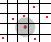
\includegraphics[scale=3]{pics/grid.png}
\caption{\emph{For each particle, only the eight neighboring squares need to be checked for collisions.}}
\label{fig:gird}
\end{figure}
\\
After creating the grid, we implemented a \emph{findNearest} function that returned all the particles in the vicinity of the input particle. In each timestep the grid had to be filled with the new positions of all particles, but this is done in $O(n)$ by simply checking each particle and now each particle only needed to be checked for collision by the ones close to it:
\\
\rule{125mm}{0.1pt}
\begin{algorithmic}
\STATE $n \gets numberOfParticles$
\FOR{$i = 0 \to n$}
	\STATE $particles[i].ax \gets 0$
	\STATE $particles[i].ay \gets 0$
	\STATE $nearParticles[] = findNearest(particles[i])$
	\FOR{$j = 0 \to nearParticles.size$}
			\STATE $apply\_force(particles[i],nearParticles[j])$
	\ENDFOR
\ENDFOR 
\end{algorithmic}
\rule{125mm}{0.1pt}
\vspace{10pt}
\\
Since the particles are evenly distributed over the area, \emph{nearParticles.size} will rarely be greater than one (only in the case of a particle colliding with multiply others in the same timestep) and thus we had reduced the algorithm to $O(n)$.

\subsection{Pthreads}
When adapting this solution to be able to run parallel with \emph{pthreads} a slight change was needed: we split the particles up in a way so that each thread only checked collisions for a range of particles depending on the thread's id. Thus dividing the workload evenly.
\\
\rule{125mm}{0.1pt}
\begin{algorithmic}
\STATE $first \gets min(thread\_id * particles\_per\_thread,n)$
\STATE $last \gets min((thread\_id+1) * particles\_per\_thread,n)$
\STATE $n \gets numberOfParticles$
\FOR{$i = first \to last$}
	\STATE $particles[i].ax \gets 0$
	\STATE $particles[i].ay \gets 0$
	\STATE $nearParticles[] = findNearest(particles[i])$
	\FOR{$j = 0 \to nearParticles.size$}
			\STATE $apply\_force(particles[i],nearParticles[j])$
	\ENDFOR
\ENDFOR 
\end{algorithmic}
\rule{125mm}{0.1pt}
\vspace{10pt}
\\
Where $particles\_per\_thread = (n+numThreads-1)/numThreads$. By having a barrier at the end of this section of code we also guaranteed that no thread would finish and start moving particles in the next timestep while others where still working.
\subsection{OpenMP}
To adapt the solution to be run in parallel in OpenMP we had the same approach of dividng up the particles checked between the threads. However, in OpenMP this was done much easier by simply using \emph{omp for}:
\\
\rule{125mm}{0.1pt}
\begin{algorithmic}
\STATE $n \gets numberOfParticles$
\STATE $\#pragma\;omp\;for$
\FOR{$i = 0 \to n$}
	\STATE $particles[i].ax \gets 0$
	\STATE $particles[i].ay \gets 0$
	\STATE $nearParticles[] = findNearest(particles[i])$
	\FOR{$j = 0 \to nearParticles.size$}
			\STATE $apply\_force(particles[i],nearParticles[j])$
	\ENDFOR
\ENDFOR 
\end{algorithmic}
\rule{125mm}{0.1pt}
\vspace{10pt}
\\
Since the grid was shared among the threads, we also had to make sure that it was only filled by one of the threads using \emph{\#pragma omp single} to avoid segmentation faults when adding particles.
\subsection{MPI}
Since we are unable to have global data accessable among the processes when using MPI, we had to collect all global data locally at the beginning of every timestep using the \emph{MPI\_Allgatherv} function. Each process had a local array containing the particles it was responsible for checking, this was (just as when using pthreads) calculated using the processe's \emph{rank} and the number of processes. Thus, the collision checking loop only checked the particles contained in its local array:
\\
\rule{125mm}{0.1pt}
\begin{algorithmic}
\STATE $nlocal\quad //size\;of\;local\;array$
\STATE $local[]\quad //particles\;recieved\;from\;MPI\_Allgatherv$
\FOR{$i = 0 \to nlocal$}
	\STATE $local[i].ax \gets 0$
	\STATE $local[i].ay \gets 0$
	\STATE $nearParticles[] = findNearest(local[i])$
	\FOR{$j = 0 \to nearParticles.size$}
			\STATE $apply\_force(local[i],nearParticles[j])$
	\ENDFOR
\ENDFOR 
\end{algorithmic}
\rule{125mm}{0.1pt}
\vspace{10pt}
\\
\newpage
\section{Results}
In this section, the results are presented in charts to easily demostrate speed improvements. A full list containing the data can be found in the apendix.
\subsection{Serial}
The results from our version of the serial implementation clearly showed that we had managed to improve the algorithm to run in $O(n)$. \\
\begin{center}
    \begin{tabular}{ | l | l | l |}
    \hline
    Num Particles & $O(n)$ & $O(n^{2})$  \\ \hline
    100 & 0.06s & 0.06s  \\ \hline
    500 & 0.3s & 1.08s  \\ \hline
    1000 & 0.6s & 4.79s  \\ \hline
    2000 & 1.19s & 19.1s \\
    \hline
    \end{tabular}
\end{center}
\begin{figure}[htb]
\centering
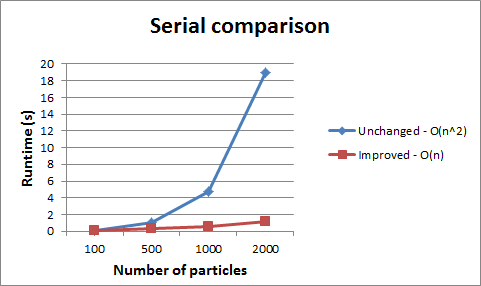
\includegraphics[scale=1]{pics/serial.png}
\caption{\emph{Comparison between the given algorithm and our improved version.}}
\label{fig:gird}
\end{figure}
\subsection{Pthreads}
Looking at the results from our pthreads implementation, we saw that we had been successful in parallelising our algorithm. \newpage
\vspace{10pt}
\begin{figure}[htb]
\centering
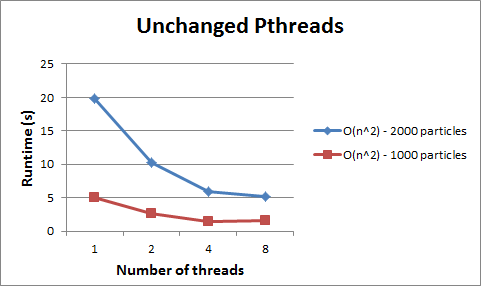
\includegraphics[scale=0.8]{pics/pth1.png}
\caption{\emph{Runtime of the given pthreads-implementation depending on number of threads and particles.}}
\label{fig:gird}
\end{figure}
\vspace{10pt}

\begin{figure}[htb]
\centering
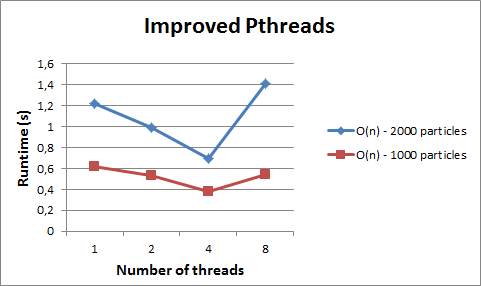
\includegraphics[scale=0.8]{pics/pth2.png}
\caption{\emph{Runtime of our pthreads-implementation depending on number of threads and particles.}}
\label{fig:gird}
\end{figure}
\newpage
\subsection{OpenMP}
\begin{figure}[h!]
\centering
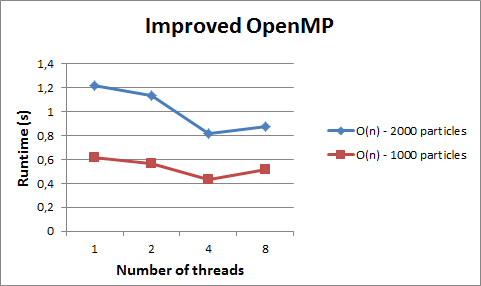
\includegraphics[scale=0.8]{pics/open1.png}
\caption{\emph{Runtime of our OpenMP-implementation depending on number of threads and particles}.}
\label{fig:gird}
\end{figure}
\subsection{MPI}
\begin{figure}[h!]
\centering
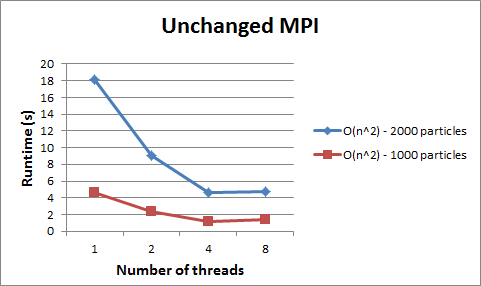
\includegraphics[scale=0.8]{pics/mpi1.png}
\caption{\emph{Runtime of the given MPI-implementation depending on number of threads and particles.}}
\label{fig:gird}
\end{figure}

\begin{figure}[htb]
\centering
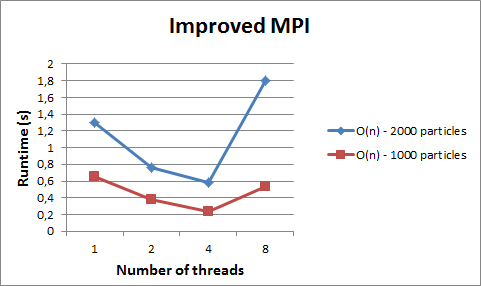
\includegraphics[scale=0.8]{pics/mpi2.png}
\caption{\emph{Runtime of our MPI-implementation depending on number of threads and particles.}}
\label{fig:gird}
\end{figure}

\newpage
\section{Discussion}
As can be clearly seen from even a quick glance at the graphs in the result-section the biggest performance gain was achieved not from parallelization but from improving the time complexity of the algorithm, from $O(n^{2})$ to $O(n)$. When running the $O(n^{2})$ algorithm on a set of 2000 particles it requires circa 19.1 seconds to complete. The corresponding figure for the $O(n)$ algorithm is circa 1.2 seconds, a performance increase of a staggering 1592 percent. Meanwhile, the maximum performance increase gained from parallelizing was only (using pthreads and 4/4 cores) 335 percent. Indeed, the performance gain will be bigger in systems with more cores, but Amdahl's law tells us that as the amount of cores grow we will see diminishing returns in terms of performance boost.

So does this all make sense? Can we lean back and say "yes, this seems about right"? Lets have a look at what the mathematics tells us. First, Amdahl's law says that the maximum performance gain will be $speedup = 1/(s+((1 - s)/n)$, where $s = the percentage of the program that is sequential$ and $n = the number of cores used$. We cant be sure of the value of $s$ in our case so we are going to calculate it using the above formula. The speedup gained by going from 1 to 4 cores was approximately 3.35, so we have that $3.35 = 1/(s+((1 - s)/4)$ which gives $s = 0.065$. With that in mind, lets see how much speedup we can expect from a massive multi core system, with lets say 128 cores. Setting $n = 128$ gives us a speedup of around 13.8 times. This is indeed quite the performance gain but it is massively dwarfed by the performance gain given by the improved algorithm, where the time complexity decreases with the square root, from quadratic lo linear! This is backed up by the fact that $lim x -> inf sqr(n)/(s+((1 - s)/n)^{-1} = sqr(n)$. All in all we are hence not surprised by the results and find them to be quite as expected.

Lets be content with that and move on to assume that the algorithm cannot be improved any more, and the only remaining source for performance boosts will be from parallelization. The different libraries used  all have their pros and cons. Using the posix native pthreads library is convenient because it doesn't require any third-party library, that keeps things simple enough from a development point of view. OpenMP on the other hand provides unrivaled simplicity and will actually compile on computers without it because of the use of the \#pragma directives. MPI was interesting because it was the only message passing library we used, it was also the quickest by a bit. Furthermore MPI can be used not only for multi threading in the same chip, but also across computers so that clusters can be built. This provides for a simple way to scale the application in a way that the other libraries cannot match.

At the end of the day we would probably decide to use OpenMP, if nothing else for its sheer simplicity which is simply unrivaled. We feel that developing a parallel application with OpenMP will be a lot quicker than with any of the other libraries, even for experienced developers, and time is as you know money. Yes, sure, our tests say that it is the slowest of the three but only by a little bit, in fact the difference between OpenMP and pthreads probably lies within the error margin.
\section{Appendix}
All programs were deceloped and tested on a x86\_64 Intel Core Quad Q9400 running Red Hat Enterprise Linux 5.6. All code was compiled and linked with gcc 4.1.2. 
\end{document}
